%% 第2章 AI Agent 智能体编排系统需求分析

\chapter{AI Agent 智能体编排系统需求分析}

\section{系统功能需求分析}

\subsection{功能需求描述}

系统面向三类用户角色：Java 开发者（API 集成与配置）、业务人员（可视化编排与审批）
和系统管理员（运维与监控）。系统用例图如图~\ref{fig:use_case}~所示。

\begin{figure}[H]
  \centering
  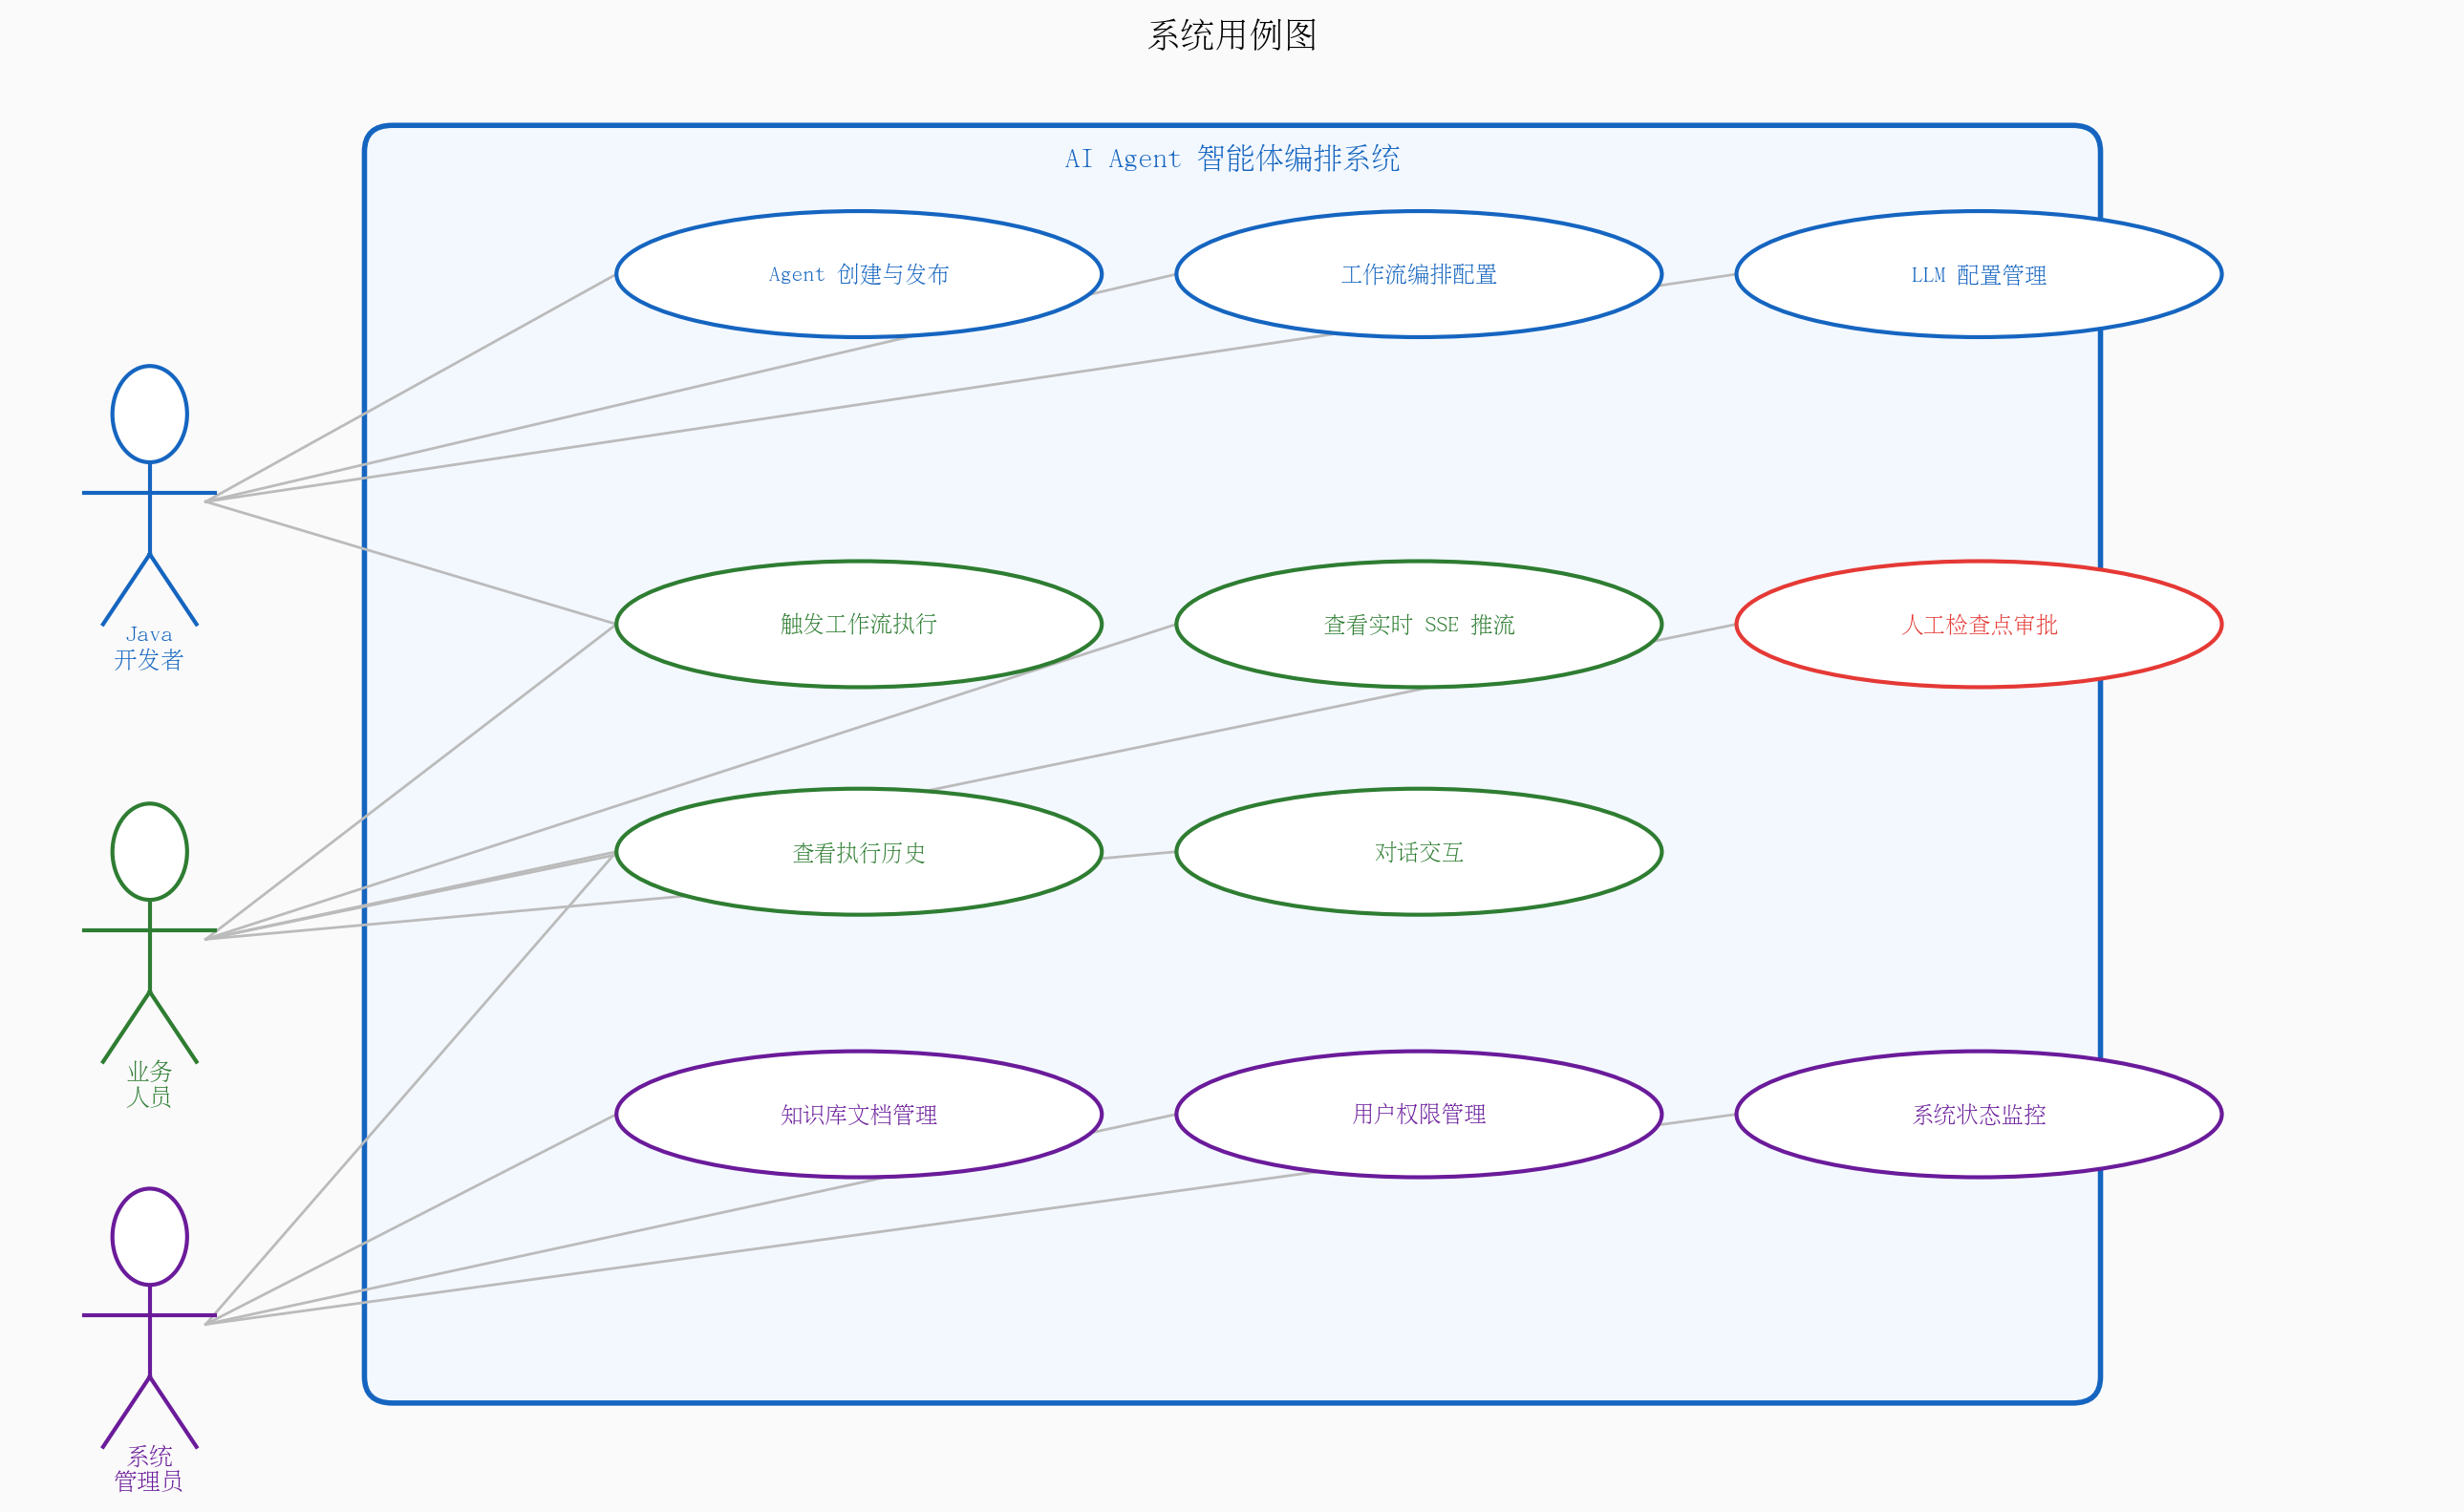
\includegraphics[width=0.95\textwidth]{figures/fig_usecase.png}
  \caption{系统用例图}
  \label{fig:use_case}
\end{figure}

围绕论文最终确定的五个核心模块，系统功能需求可归纳如下：

\subsubsection{（1）Agent 管理与可视化编排需求}

系统需要支持 Agent 的全生命周期管理，包括创建、编辑、发布、版本查询与回滚。
用户可维护 Agent 的基础信息（名称、描述、图标）以及底层工作流图定义。
在前端，业务人员通过可视化画布拖拽节点、配置参数、建立边连接，
并将画布状态保存为 JSON 图结构。系统需保证草稿态与发布态隔离，
避免开发中的修改直接影响线上运行中的 Agent。

\subsubsection{（2）工作流调度执行需求}

系统需要支持基于 DAG 的工作流执行能力。用户在对话界面输入任务后，
系统应根据 Agent 配置解析工作流图，完成节点状态初始化、拓扑调度、条件分支处理、
并行节点执行和最终结果汇总。执行过程中需要实时输出节点运行进度和模型生成结果，
并保证执行状态可查询、执行日志可追溯。

\subsubsection{（3）人工审核与恢复机制需求}

系统需要在关键节点引入人工检查点机制。当工作流执行到指定节点时，
可根据 BEFORE\_EXECUTION 或 AFTER\_EXECUTION 两种阶段自动暂停，
等待审批人查看输入或输出内容后进行决策。审批人可通过审批页面选择通过或拒绝，
并在通过前对中间结果进行修正。系统需记录审批人、审批时间、修改内容和拒绝原因，
满足合规审计要求，同时在多人并发审批时保障状态一致性。

\subsubsection{（4）知识库与检索增强需求}

系统需要支持知识数据集管理、文档上传、分块处理、向量化入库和检索增强。
用户可上传 PDF、Word、TXT、Markdown 等多种格式文档，系统对文档进行解析与分块后，
调用嵌入模型将文本块写入 Milvus 向量数据库。运行时，工作流中的知识节点或检索接口
应能够根据用户问题进行语义搜索，返回 Top-K 相关内容作为上下文，增强大模型回答质量。

\subsubsection{（5）用户认证与系统安全支撑需求}

系统需要提供用户注册、登录、找回密码和身份认证能力。
注册与重置密码需依赖邮箱验证码校验；登录后系统应签发访问令牌，
保证 Agent 管理、知识库管理、工作流执行与审批操作均运行在已认证用户上下文中。
同时，系统应具备验证码发送频率限制、登录失败限流、密码加密存储和访问审计等安全能力。

\subsection{主要用例详细描述}

在系统所有功能中，Agent 管理与编排、工作流执行、人工审核、知识检索和用户认证构成了核心闭环。
以下选取其中五个代表性用例进行详细说明。

\subsubsection{（1）Agent 创建与发布}

表~\ref{tab:uc_agent}~为 Agent 创建与发布用例的需求说明表。

\begin{table}[H]
  \centering
  \caption{Agent 创建与发布用例需求表}
  \label{tab:uc_agent}
  \begin{tabular}{|p{3cm}|p{10cm}|}
    \hline
    \textbf{用例标识} & UC-01 Agent 创建与发布 \\
    \hline
    \textbf{功能描述} & 用户创建 Agent、在可视化画布中完成编排并发布可执行版本 \\
    \hline
    \textbf{使用人员} & Java 开发者 / 业务人员 \\
    \hline
    \textbf{前置条件} & 用户已登录，具有 Agent 管理权限 \\
    \hline
    \textbf{输入} & Agent 基础信息、节点配置、边连接关系、图结构 JSON \\
    \hline
    \textbf{系统响应} & 创建初始 Agent，保存 graphJson，校验图结构并生成版本快照 \\
    \hline
    \textbf{输出} & 返回 Agent ID、最新版本信息和发布结果 \\
    \hline
    \textbf{操作序列} & 用户创建 Agent 并进入画布编排，保存草稿后发布版本，系统写入版本快照 \\
    \hline
    \textbf{异常} & 图结构存在环路 → 拒绝保存；版本冲突 → 提示重新加载草稿 \\
    \hline
  \end{tabular}
\end{table}

\subsubsection{（2）工作流执行}

表~\ref{tab:uc_exec}~为工作流执行用例的需求说明表。

\begin{table}[H]
  \centering
  \caption{工作流执行用例需求表}
  \label{tab:uc_exec}
  \begin{tabular}{|p{3cm}|p{10cm}|}
    \hline
    \textbf{用例标识} & UC-02 工作流执行 \\
    \hline
    \textbf{功能描述} & 用户输入任务，触发 Agent 工作流执行，实时接收 SSE 推送的进度和结果 \\
    \hline
    \textbf{使用人员} & Java 开发者 / 业务人员 \\
    \hline
    \textbf{前置条件} & Agent 已发布，工作流配置完整，DAG 无环 \\
    \hline
    \textbf{输入} & 用户消息（input/query/message）、agentId、conversationId（可选） \\
    \hline
    \textbf{系统响应} & 解析 Agent 图定义，加载检索增强上下文与会话历史，初始化执行上下文，DAG 拓扑调度 \\
    \hline
    \textbf{输出} & 通过 SSE 推送节点启动/完成/错误事件和 LLM 流式输出 delta；执行完成后返回最终结果 \\
    \hline
    \textbf{操作序列} & 用户发送消息后建立 SSE 连接，调度器按图结构执行节点并持续推送执行事件 \\
    \hline
    \textbf{异常} & 节点执行失败 → 推送 error 事件，整体状态变为 FAILED；DAG 含环 → start() 抛异常，返回 400 \\
    \hline
  \end{tabular}
\end{table}

图~\ref{fig:exec_flow}~展示了工作流执行的完整流程。

\begin{figure}[H]
  \centering
  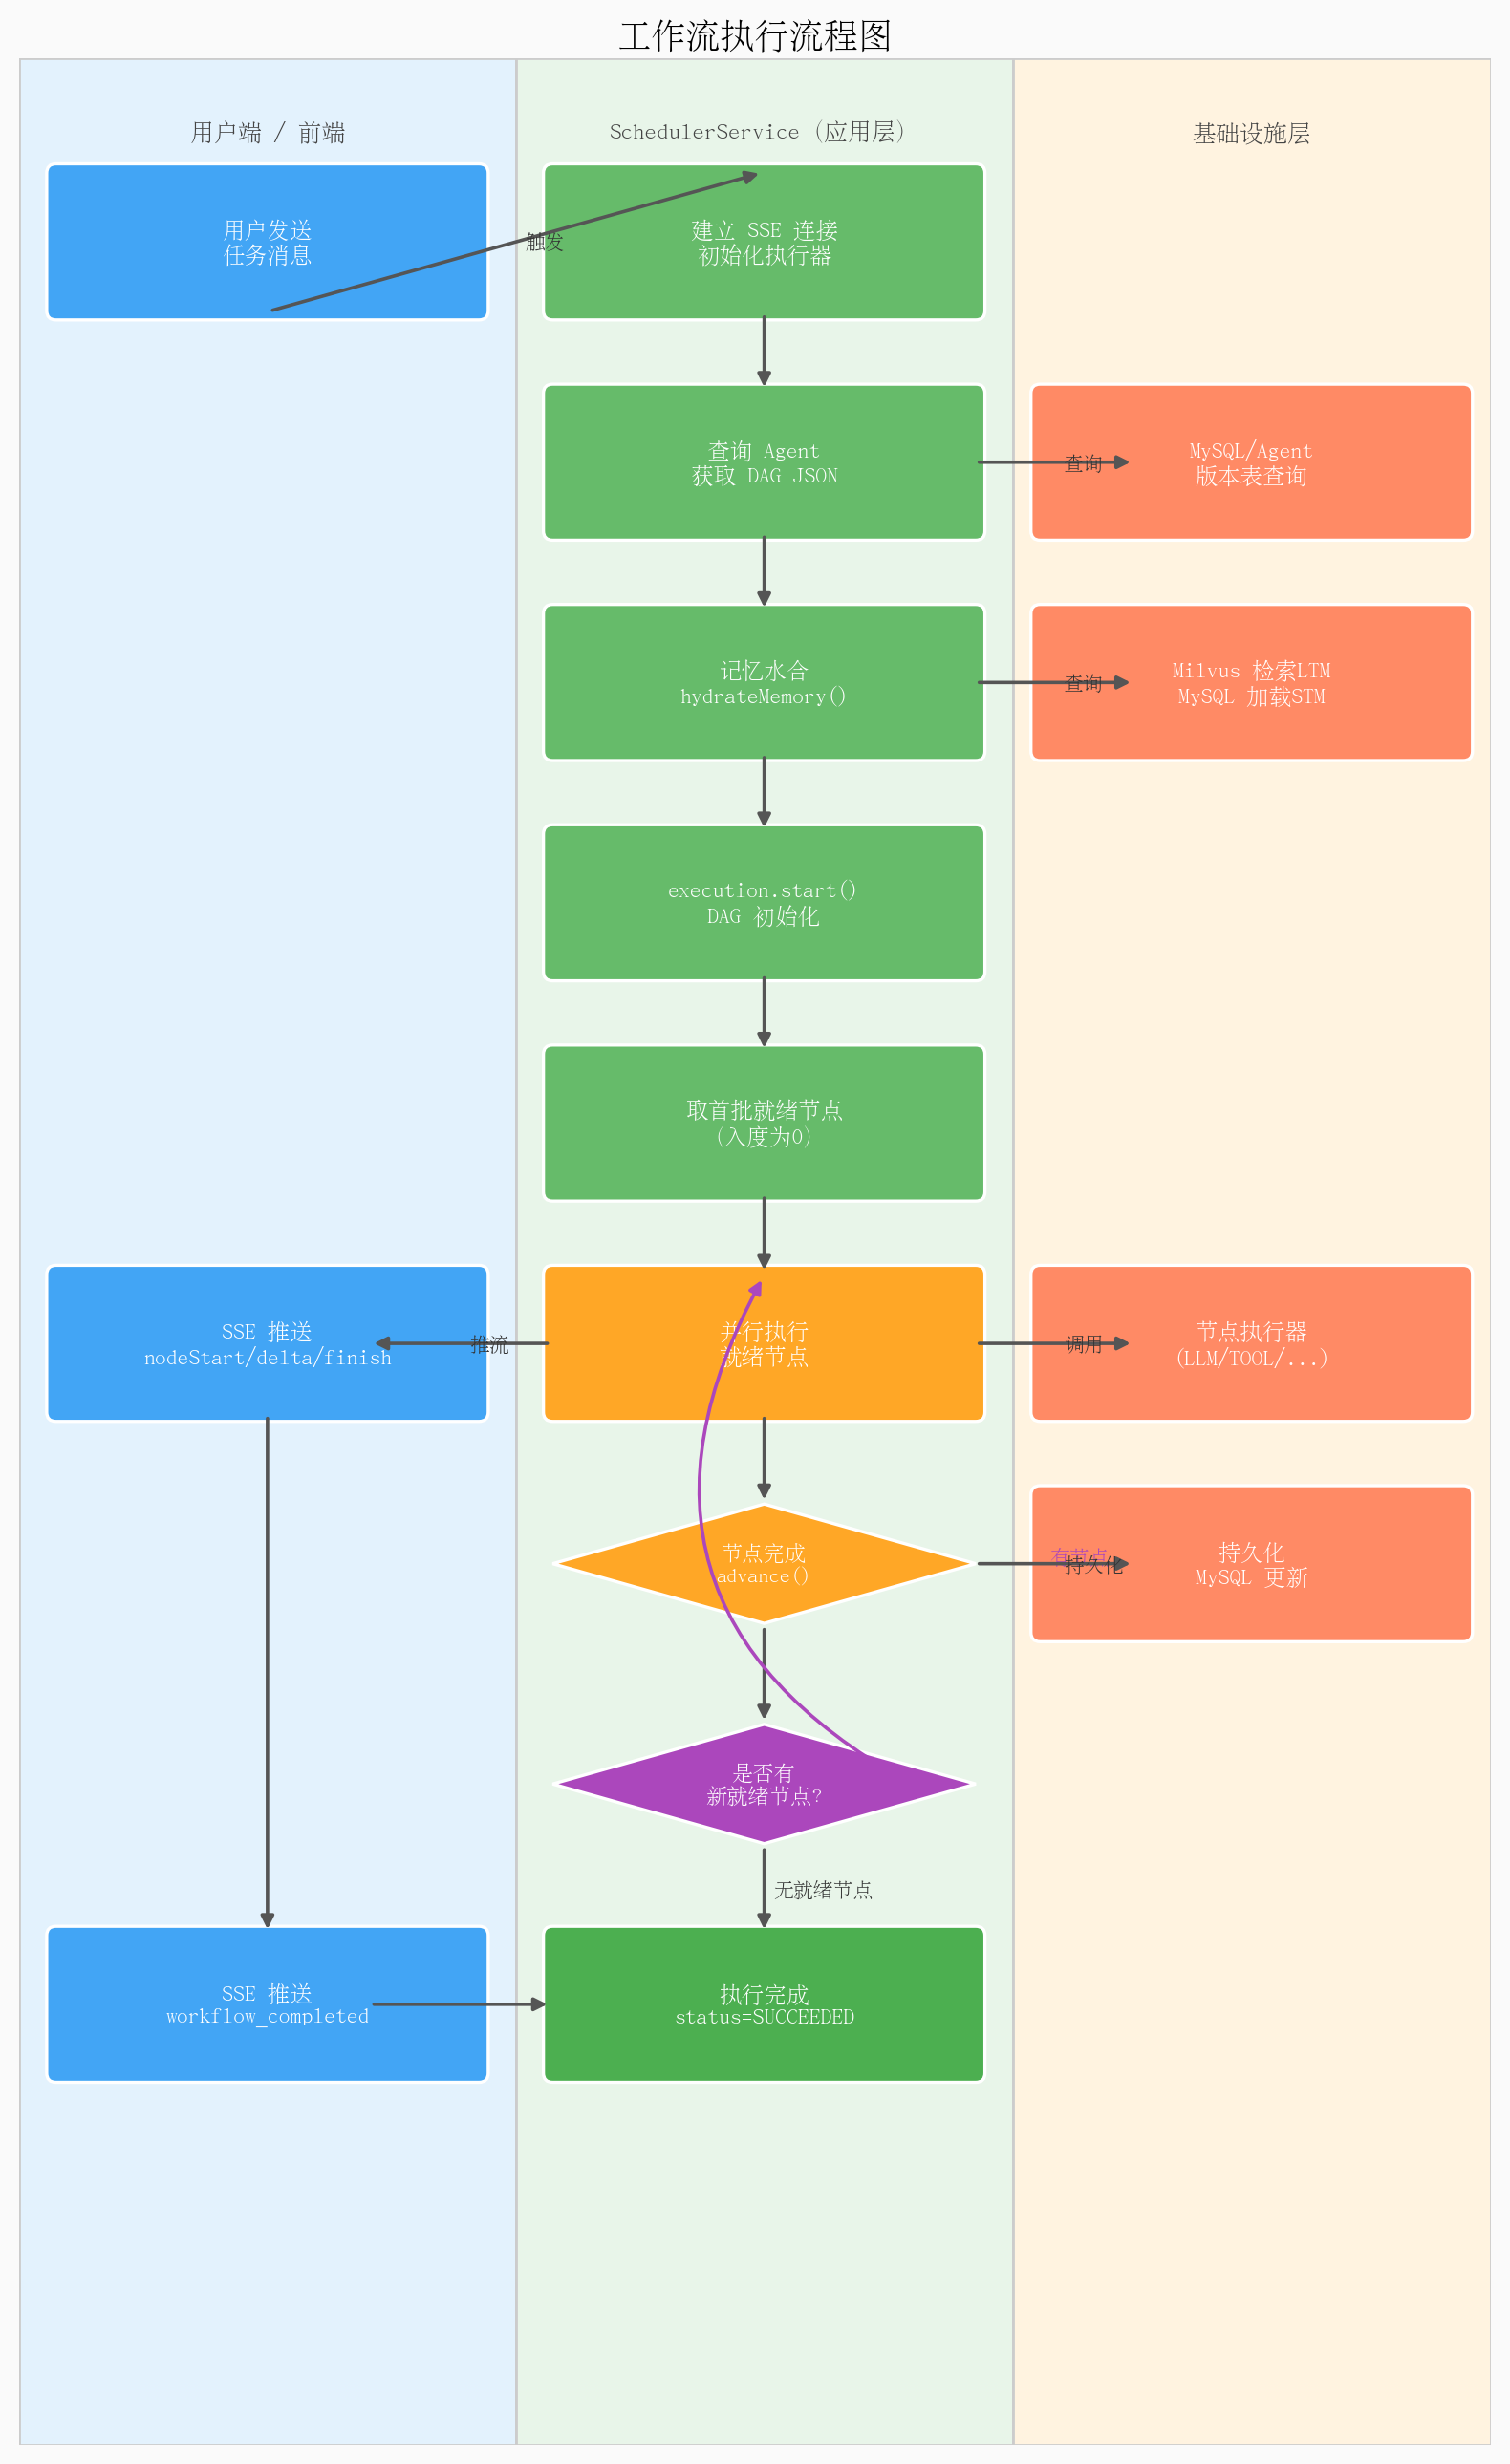
\includegraphics[width=0.68\textwidth]{figures/fig_exec_flow.png}
  \caption{工作流执行流程图}
  \label{fig:exec_flow}
\end{figure}

用户在前端对话界面输入消息后，前端建立 SSE 连接并调用工作流启动接口，
系统首先从向量数据库检索与用户输入语义相关的知识片段，
再从会话存储中加载最近的对话历史，
将两者注入执行上下文后调用 \texttt{execution.start(inputs)} 初始化 DAG。
调度器依次取出就绪节点（入度为 0 的节点）并发执行，
每个节点完成后调用 \texttt{advance()} 推进状态，计算下一批就绪节点，
直至所有节点完成，整体状态更新为 \texttt{SUCCEEDED}。

\subsubsection{（3）人工检查点审批}

表~\ref{tab:uc_review}~为人工审批用例的需求说明表。

\begin{table}[H]
  \centering
  \caption{人工检查点审批用例需求表}
  \label{tab:uc_review}
  \begin{tabular}{|p{3cm}|p{10cm}|}
    \hline
    \textbf{用例标识} & UC-03 人工检查点审批 \\
    \hline
    \textbf{功能描述} & 工作流执行到配置了人工检查点的节点时自动暂停，审批人查看并决策后工作流继续运行 \\
    \hline
    \textbf{使用人员} & 业务人员 / 系统管理员 \\
    \hline
    \textbf{前置条件} & 工作流执行状态为 PAUSED\_FOR\_REVIEW，存在待审批记录 \\
    \hline
    \textbf{输入（通过）} & executionId、nodeId、expectedVersion、可选的 edits（修改内容）、comment \\
    \hline
    \textbf{输入（拒绝）} & executionId、nodeId、expectedVersion、reason（拒绝原因） \\
    \hline
    \textbf{系统响应} & 通过乐观锁校验版本，合并编辑内容，写审批记录，更新执行状态 \\
    \hline
    \textbf{输出（通过）} & 执行恢复（RUNNING），SSE 推送 workflow\_resumed，后续节点继续调度 \\
    \hline
    \textbf{输出（拒绝）} & 执行终止（FAILED），SSE 推送 workflow\_rejected，写拒绝审批记录 \\
    \hline
    \textbf{操作序列} & 执行暂停后前端展示审批面板，审批人决策后系统更新状态并通过 SSE 通知前端 \\
    \hline
    \textbf{异常} & 并发审批（version 不匹配）→ 返回 409 Conflict；节点不匹配 → 返回 400 \\
    \hline
  \end{tabular}
\end{table}

图~\ref{fig:review_flow}~展示了人工检查点的完整流程。

\begin{figure}[H]
  \centering
  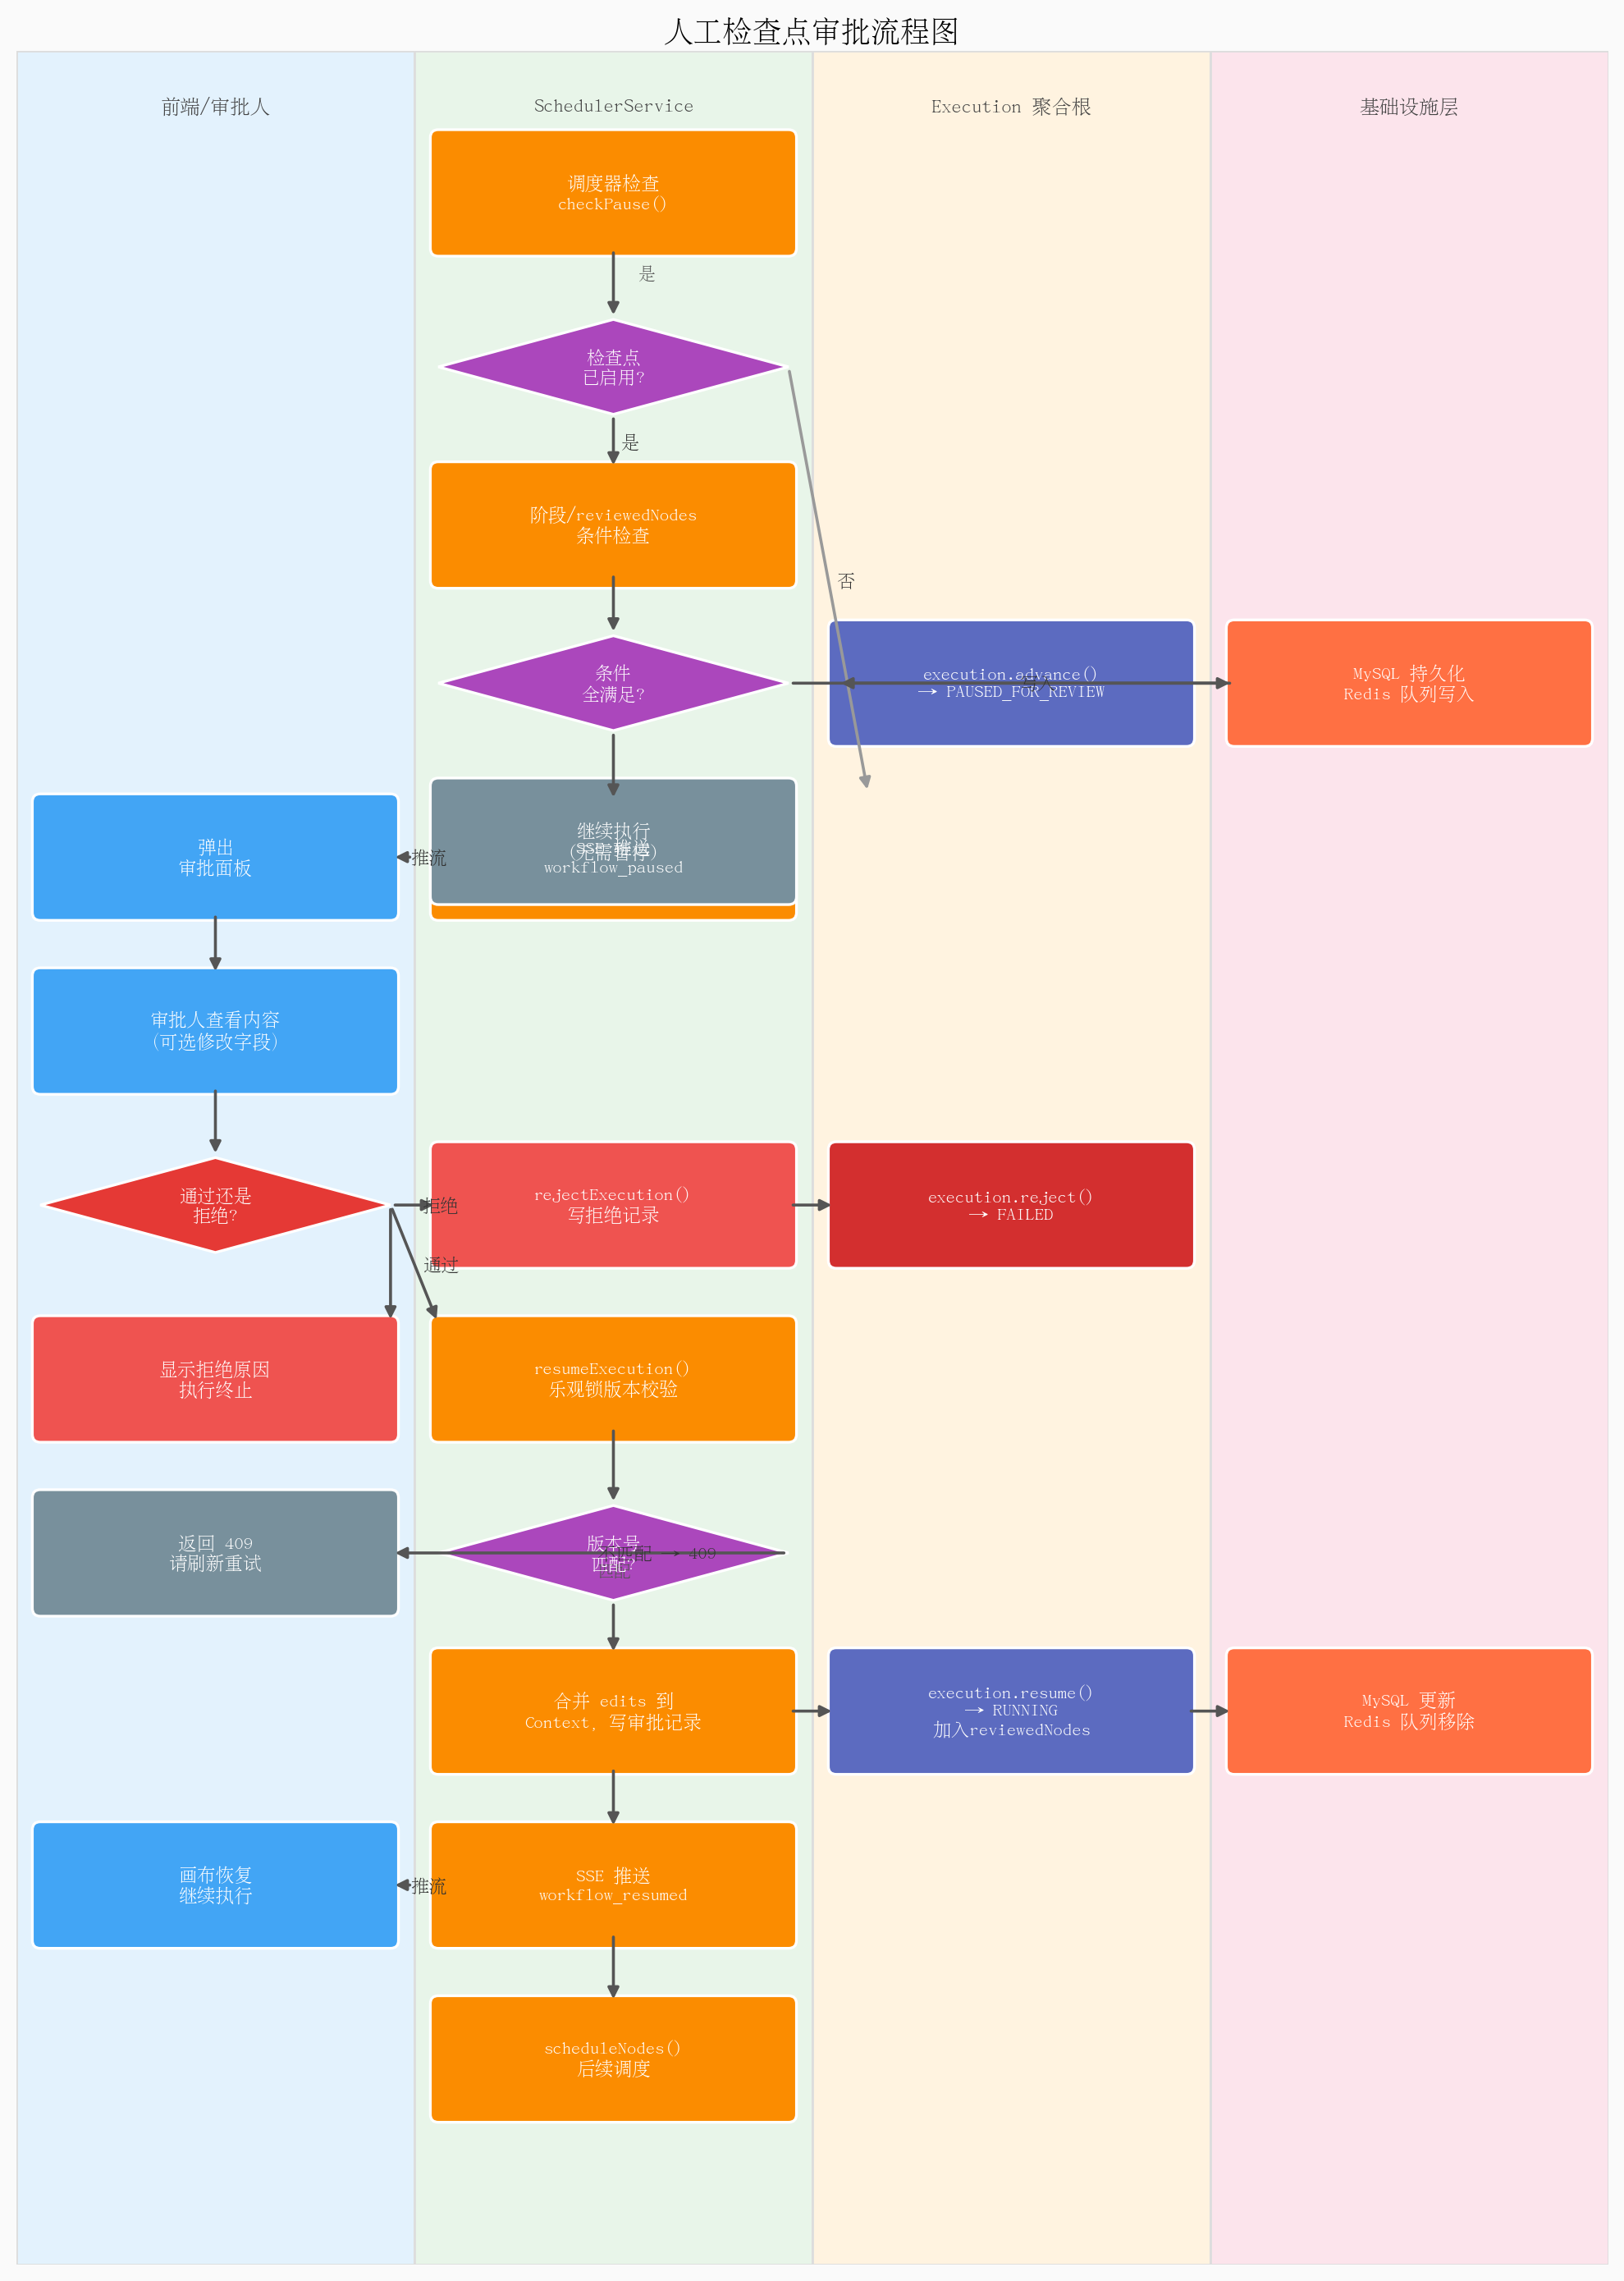
\includegraphics[width=0.72\textwidth]{figures/fig_review_flow.png}
  \caption{人工检查点审批流程图}
  \label{fig:review_flow}
\end{figure}

当执行到配置了检查点的节点时，系统通过 SSE 向前端推送 \texttt{workflow\_paused} 事件，
前端弹出审批面板，展示当前节点的输入（\texttt{BEFORE\_EXECUTION}）
或输出（\texttt{AFTER\_EXECUTION}）内容。
审批人检查内容后，若认为结果需要修正，可直接在面板中编辑字段值；
点击"通过"后，前端携带 \texttt{expectedVersion}（乐观锁）和修改内容提交，
服务端校验版本一致性，合并编辑内容到上下文，写入审批记录，之后恢复工作流执行。
若审批人点击"拒绝"，则工作流立即终止，审批记录中写入拒绝原因。

\subsubsection{（4）知识库检索增强}

表~\ref{tab:uc_knowledge}~为知识库检索增强用例的需求说明表。

\begin{table}[H]
  \centering
  \caption{知识库检索增强用例需求表}
  \label{tab:uc_knowledge}
  \begin{tabular}{|p{3cm}|p{10cm}|}
    \hline
    \textbf{用例标识} & UC-04 知识库检索增强 \\
    \hline
    \textbf{功能描述} & 用户上传文档形成知识库，工作流在运行时根据查询语义召回相关片段增强模型上下文 \\
    \hline
    \textbf{使用人员} & 业务人员 / 系统管理员 / 系统（自动检索） \\
    \hline
    \textbf{前置条件} & 知识文档已上传并完成向量化入库，Milvus Collection 已就绪 \\
    \hline
    \textbf{输入} & 文档文件、分块配置、用户查询语句 \\
    \hline
    \textbf{系统响应} & 解析文档、文本分块、调用嵌入模型写入向量库，并在运行时完成 Top-K 语义检索 \\
    \hline
    \textbf{输出} & 检索到的相关片段写入上下文，供后续 LLM 节点拼接使用 \\
    \hline
    \textbf{操作序列} & 用户上传文档后系统异步处理并向量化，运行时检索相关片段增强模型输入 \\
    \hline
    \textbf{异常} & Milvus 不可达 → 记录异常日志并降级；文档解析失败 → 文档状态标记 FAILED \\
    \hline
  \end{tabular}
\end{table}

\subsubsection{（5）用户注册与登录}

表~\ref{tab:uc_auth}~为用户注册与登录用例的需求说明表。

\begin{table}[H]
  \centering
  \caption{用户注册与登录用例需求表}
  \label{tab:uc_auth}
  \begin{tabular}{|p{3cm}|p{10cm}|}
    \hline
    \textbf{用例标识} & UC-05 用户注册与登录 \\
    \hline
    \textbf{功能描述} & 用户通过邮箱验证码完成注册，并在登录成功后获取访问令牌使用系统功能 \\
    \hline
    \textbf{使用人员} & 普通用户 / 系统管理员 \\
    \hline
    \textbf{前置条件} & 邮件服务正常，验证码缓存服务可用 \\
    \hline
    \textbf{输入} & 邮箱、验证码、密码、用户名、登录 IP \\
    \hline
    \textbf{系统响应} & 校验验证码、密码强度与账号唯一性，完成密码加密和用户身份校验 \\
    \hline
    \textbf{输出} & 注册成功返回用户信息；登录成功返回访问令牌；失败时返回错误原因 \\
    \hline
    \textbf{操作序列} & 用户获取邮箱验证码并提交注册信息，登录成功后系统签发 JWT 访问令牌 \\
    \hline
    \textbf{异常} & 验证码错误或过期 → 注册失败；密码错误次数过多 → 登录受限；邮箱重复注册 → 拒绝创建 \\
    \hline
  \end{tabular}
\end{table}

\section{非功能需求}

\subsection{性能需求}

\begin{itemize}
  \item 核心非流式接口应具备良好的实时响应能力，能够满足管理与审批场景下的交互要求
  \item SSE 执行状态推送端到端延迟应控制在秒级以内，保证前端画布和日志实时更新
  \item 调度器从节点就绪到触发执行的延迟应足够低，能够支持多节点顺畅推进
\end{itemize}

\subsection{可靠性需求}

\begin{itemize}
  \item 工作流执行状态持久化到 MySQL，历史记录可查
  \item Redis 维护待审批队列和分布式锁，乐观锁保障并发安全
  \item 文档处理状态、审批记录和执行日志均需具备可恢复、可追溯能力
\end{itemize}

\subsection{可扩展性需求}

\begin{itemize}
  \item 节点执行器采用策略模式，新节点类型只需实现 \texttt{NodeExecutorStrategy} 接口
  \item 大模型接口通过 Spring AI 统一适配，支持多厂商模型切换
  \item 知识分块策略、向量存储和邮件服务等基础能力应可替换扩展
\end{itemize}

\subsection{安全性需求}

\begin{itemize}
  \item 所有 REST API 接口通过 JWT Token 鉴权
  \item 密码需以加密哈希形式存储，禁止明文保存
  \item 验证码发送和登录失败均需具备频率限制
  \item 审批操作记录操作人（reviewerId）并持久化，满足审计合规要求
\end{itemize}

\section{本章小结}

本章围绕三类用户角色系统梳理了功能需求，
并将系统能力统一收束为 Agent 管理与可视化编排、工作流调度执行、
人工审核与恢复机制、知识库与检索增强、用户认证与系统安全支撑五个模块。
通过五个关键用例的需求表格与流程描述，明确了系统的主要交互链路，
并从性能、可靠性、可扩展性和安全性四个维度给出了非功能需求，
为后续系统设计与实现奠定了需求基础。
